\documentclass[../../main.tex]{subfiles}
\begin{document}

{\bf [解]}

% TODO: 概要図
\begin{figure}[htb]
  \centering
  \begin{tikzpicture}[x=2.2cm, y=1.2cm, >=stealth, every node/.style={font=\small}]

    % --- 1. 座標定義 ---
    % alpha = -0.5, beta = 1.3
    \def\al{-0.5}
    \def\be{1.3}
    \pgfmathsetmacro{\yP}{\al*\al}       % 0.25
    \pgfmathsetmacro{\yQ}{\be*\be}       % 1.69
    \pgfmathsetmacro{\xM}{(\al + \be)/2} % 0.4
    \pgfmathsetmacro{\yM}{(\yP + \yQ)/2} % 0.97

    \coordinate (O) at (0, 0);
    \coordinate (P) at (\al, \yP);
    \coordinate (Q) at (\be, \yQ);
    \coordinate (M) at (\xM, \yM);

    % --- 2. 座標軸 ---
    \draw[->, thick, gray!80!black] (-1.6, 0) -- (2.0, 0) node[right] {$x$};
    \draw[->, thick, gray!80!black] (0, -0.4) -- (0, 2.5) node[above] {$y$};
    \node[below left=2pt] at (O) {$O$};

    % --- 3. 放物線 y = x^2 ---
    \draw[line width=1.5pt, blue!85!black, domain=-1.4:1.5, samples=70]
    plot (\x, {\x*\x});
    \node[blue!90!black, font=\footnotesize\bfseries, above right] at (1.3, 1.8) {$y = x^2$};

    % --- 4. 弦 PQ (長さ L) ---
    \draw[line width=1.4pt, teal!85!black] (P) -- (Q)
    node[pos=0.8, above left=1pt, font=\footnotesize\bfseries] {長さ $L$};

    % --- 5. 投影点線と目盛り ---
    % 点 P
    \draw[dashed, gray!60] (\al, 0) -- (P);
    \node[below=2pt, font=\scriptsize] at (\al, 0) {$\alpha$};

    % 点 Q
    \draw[dashed, gray!60] (\be, 0) -- (Q);
    \node[below=2pt, font=\scriptsize] at (\be, 0) {$\beta$};

    % 中点 M(l, h)
    \draw[dashed, red!70!black] (\xM, 0) -- (M) -- (0, \yM);
    \node[below=2pt, font=\scriptsize, red!90!black] at (\xM, 0) {$l$};
    \node[left=2pt, font=\scriptsize, red!90!black]  at (0, \yM) {$h$};

    % 等長マーク (P-M と M-Q)
    \draw[thick, gray!70!black] ($ (P)!0.5!(M) + (-0.03, 0.05) $) -- ($ (P)!0.5!(M) + (0.03, -0.05) $);
    \draw[thick, gray!70!black] ($ (M)!0.5!(Q) + (-0.03, 0.05) $) -- ($ (M)!0.5!(Q) + (0.03, -0.05) $);

    % --- 6. 点プロットとラベル ---
    \fill[black] (P) circle (1.4pt) node[left=2pt] {$P(\alpha, \alpha^2)$};
    \fill[black] (Q) circle (1.4pt) node[right=2pt] {$Q(\beta, \beta^2)$};
    \fill[red!85!black] (M) circle (1.6pt) node[above left=1pt, font=\footnotesize\bfseries, red!90!black] {$M(l, h)$};

  \end{tikzpicture}
  \caption{放物線 $y = x^2$ 上の弦 $PQ$ とその中点 $M(l, h)$}
  \label{fig:parabola_midpoint_overview}
\end{figure}

$y=x^2$上の二点を$P(\alpha,\alpha^2)$，$Q(\beta,\beta^2)$ とおく．
ただし
\begin{align}
  \alpha<\beta \label{eq:1}
\end{align}
とおく．$PQ$の中点を$M(l,h)$とおくと
\begin{align}
  l = \dfrac{\alpha+\beta}{2}, \quad h = \dfrac{\alpha^2+\beta^2}{2} \label{eq:2}
\end{align}
である．また線分$PQ$の方程式は
\begin{align}
  PQ:y=(\alpha+\beta)x-\alpha\beta \label{eq:3}
\end{align}
である．

\paragraph{(1)}

線分$PQ$の長さ$L$と傾き$m$を表すと
\begin{align}
  \begin{cases}
    m=\alpha+\beta\\
    L=\sqrt{(\beta-\alpha)^2+(\beta^2-\alpha^2)^2}
    =(\beta-\alpha)\sqrt{1+(\alpha+\beta)^2}
  \end{cases} \label{eq:4}
\end{align}
である．第二式に第一式を代入して
\begin{align}
  \beta-\alpha = \dfrac{L}{\sqrt{1+m^2}}
\end{align}
である．よって\cref{eq:2}を変形して$m,L$を代入すると
\begin{align}
  h = \dfrac{\alpha^2+\beta^2}{2}
  =\dfrac{1}{4}\left[(\alpha+\beta)^2+(\beta-\alpha)^2\right]
  =\dfrac{1}{4}\left(m^2+\dfrac{L^2}{1+m^2}\right) \label{eq:5}
\end{align}
である．

\paragraph{(2)}

\cref{eq:4}から
\begin{align}
  \alpha\beta
  & =\dfrac{1}{4}\left[(\alpha+\beta)^2-(\beta-\alpha)^2\right]
  =\dfrac{1}{4}\left(m^2-\dfrac{L^2}{1+m^2}\right)
\end{align}
だから，$\alpha,\beta$は$x$の2次式
\begin{align}
  x^2-mx+\dfrac{1}{4}\left(m^2-\dfrac{L^2}{1+m^2}\right)=0
\end{align}
の2実解で，判別式を$D$として
\begin{align}
  D=m^2-\left(m^2-\dfrac{L^2}{1+m^2}\right)=\dfrac{L^2}{1+m^2}>0
\end{align}
となり$m$によらず$D>0$だから$m$は任意の実数値をとる．
$t=m^2$とおくとしたがって$t\ge0$である．\cref{eq:5}に代入して
\begin{align}
  h(t)=\dfrac{1}{4}\left(t+\dfrac{L^2}{1+t}\right)
\end{align}
である．この最小値を計算すれば良い．両辺$t$で微分して
\begin{align}
  h'(t)=1-\dfrac{L^2}{(1+t)^2}=\dfrac{t^2+2t+1-L^2}{(1+t)^2} = \dfrac{(t+1+L)(t+1-L)}{(1+t)^2}
\end{align}
において，$L>0$よりこの符号は$t+1-L$の符号と一致する．
よって$L$によって$h$の挙動は以下のようになる．

\subparagraph{$1^\circ$ $0<L \le 1$の時}

% TODO: h(t)の増減表
\begin{table}[htb]
  \centering
  \caption{$h(t)$ の増減表 $(0 < L \le 1)$}
  \label{tab:ht_case1}
  \renewcommand{\arraystretch}{1.5}
  \begin{tabular}{c|ccc}
    \hline
    $t$      & $0$                  & $\cdots$   & $(\to\infty)$ \\ \hline
    $h'(t)$  & $1 - L^2 \ge 0$      & $+$        &               \\ \hline
    $h(t)$   & $\dfrac{1}{4}L^2$    & $\nearrow$ & $(\to\infty)$ \\ \hline
  \end{tabular}
\end{table}

$t\ge 0$の時は$h'(t)\ge 0$で$h(t)$は単調増加になるから$t=0$で最小値
\begin{align}
  h_{\min}=h(0) = \dfrac{1}{4}L^2 \label{eq:6}
\end{align}
をとる．

\subparagraph{$2^\circ$ $1\le L$の時}

この時は$h(t)$の増減表は以下のようになる．

% TODO: upgrade
\begin{table}[htb]
  \centering
  \caption{$h(t)$ の増減表 $(1 \le L)$}
  \label{tab:ht_case2}
  \renewcommand{\arraystretch}{1.5}
  \begin{tabular}{c|ccccc}
    \hline
    $t$      & $0$               & $\cdots$   & $L-1$                     & $\cdots$   & $(\to\infty)$ \\ \hline
    $h'(t)$  & $1-L^2 \le 0$     & $-$        & $0$                       & $+$        &               \\ \hline
    $h(t)$   & $\dfrac{1}{4}L^2$ & $\searrow$ & $\dfrac{2L-1}{4}$ & $\nearrow$ & $(\to\infty)$ \\ \hline
  \end{tabular}
\end{table}

したがって$t=L-1$で最小値
\begin{align}
  \min h = h(L-1)=\dfrac{1}{4}\left[(L-1)+\dfrac{L^2}{L}\right]=\dfrac{2L-1}{4} \label{eq:7}
\end{align}
をとる．
\casesend

以上\cref{eq:6,eq:7}をまとめて求める$h$の最小値は
\begin{align}
  \min h=
  \begin{cases}
    \dfrac{1}{4}L^2&(0<L\le1)\\
    \dfrac{1}{4}(2L-1)&(1\le L)
  \end{cases}
\end{align}
である．

% TODO: min h(L)のグラフ
\begin{figure}[htb]
  \centering
  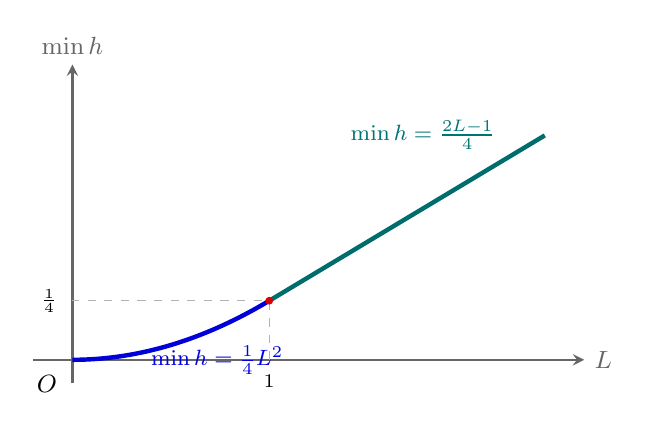
\begin{tikzpicture}[x=2.5cm, y=3.0cm, >=stealth, every node/.style={font=\small}]

    % --- 1. 座標軸 ---
    \draw[->, thick, gray!80!black] (-0.2, 0) -- (2.6, 0) node[right] {$L$};
    \draw[->, thick, gray!80!black] (0, -0.1) -- (0, 1.25) node[above] {$\min h$};
    \node[below left=2pt] at (0, 0) {$O$};

    % --- 2. 曲線・直線のプロット ---
    % 0 < L <= 1: 放物線 min h = 1/4 * L^2
    \draw[line width=1.6pt, blue!85!black, domain=0:1, samples=50]
    plot (\x, {0.25*\x*\x});

    % L >= 1: 直線 min h = 1/4 * (2L - 1) = 0.5*L - 0.25
    \draw[line width=1.6pt, teal!85!black, domain=1:2.4, samples=30]
    plot (\x, {0.5*\x - 0.25});

    % --- 3. 接続点・目盛り・補助線 ---
    % 接続点 L = 1
    \draw[dashed, gray!60] (1, 0) -- (1, 0.25) -- (0, 0.25);
    \node[below=2pt, font=\scriptsize] at (1, 0) {$1$};
    \node[left=2pt, font=\scriptsize]  at (0, 0.25) {$\frac{1}{4}$};
    \fill[red!85!black] (1, 0.25) circle (1.4pt);

    % 関数ラベル
    \node[blue!90!black, font=\footnotesize\bfseries, below right] at (0.35, 0.1)
    {$\min h = \frac{1}{4}L^2$};
    \node[teal!90!black, font=\footnotesize\bfseries, above left] at (2.2, {0.5*2.2 - 0.25})
    {$\min h = \frac{2L-1}{4}$};

  \end{tikzpicture}
  \caption{$L$ に対する中点の高さの最小値 $\min h(L)$ のグラフ}
  \label{fig:min_h_graph}
\end{figure}

\end{document}
